%%%%%%%%%%%%%%%%%%%%%%%%%%%%%%%%%%%%%%%%%%%%%%%%%%%%%%%%%%%%%%%%%%%%%%%%
%    INSTITUTE OF PHYSICS PUBLISHING                                   %
%                                                                      %
%   `Preparing an article for publication in an Institute of Physics   %
%    Publishing journal using LaTeX'                                   %
%                                                                      %
%    LaTeX source code `ioplau2e.tex' used to generate `author         %
%    guidelines', the documentation explaining and demonstrating use   %
%    of the Institute of Physics Publishing LaTeX preprint files       %
%    `iopart.cls, iopart12.clo and iopart10.clo'.                      %
%                                                                      %
%    `ioplau2e.tex' itself uses LaTeX with `iopart.cls'                %
%                                                                      %
%%%%%%%%%%%%%%%%%%%%%%%%%%%%%%%%%%
%
%
% First we have a character check
%
% ! exclamation mark    " double quote
% # hash                ` opening quote (grave)
% & ampersand           ' closing quote (acute)
% $ dollar              % percent
% ( open parenthesis    ) close paren.
% - hyphen              = equals sign
% | vertical bar        ~ tilde
% @ at sign             _ underscore
% { open curly brace    } close curly
% [ open square         ] close square bracket
% + plus sign           ; semi-colon
% * asterisk            : colon
% < open angle bracket  > close angle
% , comma               . full stop
% ? question mark       / forward slash
% \ backslash           ^ circumflex
%
% ABCDEFGHIJKLMNOPQRSTUVWXYZ
% abcdefghijklmnopqrstuvwxyz
% 1234567890
%
%%%%%%%%%%%%%%%%%%%%%%%%%%%%%%%%%%%%%%%%%%%%%%%%%%%%%%%%%%%%%%%%%%%
%
\documentclass[10pt]{iopart}
%\documentclass[12pt]{iopart}
%\newcommand{\gguide}{{\it Preparing graphics for IOP Publishing journals}}
%Uncomment next line if AMS fonts required
%\usepackage{iopams}
\usepackage{graphicx}
\usepackage{multirow}
\usepackage{color,soul}
\begin{document}

\title[Defect engineering using microwave processing in SiC and GaAs]{Defect engineering using microwave processing in SiC and GaAs}

\author{Oleg Olikh$^1$\footnote{Author to whom any correspondence should be addressed.}, Petro Lytvyn$^2$}

\address{$^1$Physics Faculty, Taras Shevchenko National University of Kyiv, Kyiv 01601, Ukraine}
\address{$^2$V. Lashkaryov Institute of Semiconductor Physics of NAS of Ukraine, Kyiv 03028, Ukraine}
\ead{olegolikh@knu.ua}
%\vspace{10pt}
%\begin{indented}
%\item[]August 2017
%\end{indented}

\begin{abstract}
The influence of microwave radiation (2.45~GHz, 1.5~W/cm$^2$, up to 80~s) on defects was studied in single crystals of $n$-6H–SiC, $n$-GaAs, and epi-GaAs.
The capture cross section of the charge carrier was found to change,
and defect complexes were reconstructed because of the growing number of  interstitial atoms in the near-surface layer.
The correlation between the changes in the defect subsystem and deformation of the near-surface layer was analyzed.
The possible mechanisms of the revealed effects are also discussed.
\end{abstract}

%
% Uncomment for keywords
\vspace{2pc}
\noindent{\it Keywords}: microwave, defect, SiC, GaAs

% Uncomment for Submitted to journal title message
\submitto{\SST}
%
% Uncomment if a separate title page is required
%\maketitle

% For two-column output uncomment the next line and choose [10pt] rather than [12pt] in the \documentclass declaration
\ioptwocol
%


\section{Introduction}\label{sec:Int}

Microelectronics is currently a field of primary importance, and  the investigation of how semiconductors and their structural properties change under the action of various external factors has become one of the most important tasks in material science.
%Numerous theoretical and experimental studies have aimed to reveal the degradation mechanisms of microelectronic devices and to develop new technologies for their production.
Numerous theoretical and experimental studies have aimed to reveal the degradation mechanisms of
\hl{semiconductor structures and to develop new technologies for microelectronic devices improvement}.
The influence of certain factors, for example, radiation, has been studied quite well --- see, for instance, \cite{KozlovsEn,RadiationEffectsBook,DefByIon}.
At the same time, new agents begin to attract more attention, such as ultrasound loading (USL) \cite{Olikh2018JAP,Olikh2006TPL},
or microwave treatment (MWT) \cite{MW:Rev,ZOHM2000,BHUNIA1998,Bacherikov2003En,Pashkov1994En,
BoltovetsEn,Milenin1994En,BelyaevIntac,ASHKINADZE1996,ProcSPIE,Belyaev1998JTFEn,
Bacherikov2008En,Konakova2015En,Konakova2012FTPEn}.
The MWT has been widely applied owing to its capability of heating solid bodies \cite{MW:Rev,ZOHM2000}.
This approach is unique because of its high efficiency and capability to increase the temperature
of a sample as a whole or at selected locations with extremely high heating speeds \cite{MW:Rev}.
As a result, MWTs are widely used to synthesize various materials, and \hl{semiconductor} compounds including \cite{MW:Rev,BHUNIA1998}.
However, this type of external influence also causes changes in the  characteristics of semiconductor materials and device structures.
For instance, it has been found that irradiation by superhigh-frequency electromagnetic waves causes relaxation of internal stresses and modification of near-surface regions
in GaAs and InP structures \cite{BoltovetsEn,Pashkov1994En,Milenin1994En,BelyaevIntac,ProcSPIE,Konakova2015En,Konakova2012FTPEn},
leveling of surface microrelief in SiC/SiO$_2$ structures \cite{Bacherikov2003En},
redistribution of impurities \cite{Bacherikov2003En,Belyaev1998JTFEn,Konakova2015En},
re--charge of complexes \cite{Milenin1994En}
and generation of defects \cite{Belyaev1998JTFEn}.
%change in charge state in the complexes \cite{Milenin1994En} and generation of defects \cite{Belyaev1998JTFEn}.
%One of the consequences of structure-admixture ordering  is a decrease in the range of
%Schottky diode parameter spread \cite{Milenin1994En,Belyaev1998JTFEn}.
\hl{The microwave-induced restructuring of impurity defects leads to
a decrease} in the spread of the Schottky diode parameters \cite{Milenin1994En,Belyaev1998JTFEn}.
Moreover, MWT has been found to induce changes in the properties of Ti, Gd, and Er films deposited on silicon carbide \cite{Bacherikov2008En},
as well as in the reconstruction of GaAs photoluminescence spectra \cite{BelyaevIntac,ProcSPIE,Belyaev1998JTFEn},
and the effect depends on both the type of dopant and the crystal structure orientation of the samples.
Overall, these facts allow us to consider the MWT as one of the most promising ways to modify semiconductor devices.

However, it is well known that the properties of semiconductor structures are significally influenced by their defect subsystem.
Defects in SiC and GaAs have been investigated extensively \cite{SiCDavid,SiCWei,GAPel2020,GASobolev2020}.
At the same time,
more detailed information regarding the MWT influence on the deep level parameters is practically unknown.
The aim of this study was to investigate the impact of MWT on the defects located in the near-surface region
of $n$--6H--SiC and $n$--GaAs single crystals,
and  GaAs  epitaxial structures.
The  acoustoelectric  transient spectroscopy was used to characterize the deep levels.
%At the same time,
%more detailed information regarding the MWT influences the deep-center parameters is practically unknown.
%The aim of this study was to investigate the impact of MWT on the parameters of deep centers located in the near-surface region of $n$–-6H-–SiC and $n$-–GaAs single crystals,
%as well as on  GaAs  epitaxial structures, using acoustoelectric  transient spectroscopy.

\section{Experimental details}\label{sec:Exp}

It has been reported \cite{BoltovetsEn,Milenin1994En,BelyaevIntac,ASHKINADZE1996,ProcSPIE} that
the impact of MWT on semiconductor structures depends on many factors.
The primary factors are the initial level of structural perfectness, conductivity, dielectric permittivity, and structural topology.
To estimate the effect of MWT on the defect parameters, we selected different samples based on the doping degree, initial level of residual mechanical stress, and structure.
They were as follows.

\noindent
i)~Single-crystal $n$--6$H$--SiC wafers were grown using the Leli method and were doped with nitrogen.
   The samples were  490~$\mu$m-thick plates with dimensions of $5\times10$~mm$^2$ and  carrier concentration $n=(3-6)\times10^{18}$~cm$^{-3}$
    (further on SIC1 and SIC2);
    and 460~$\mu$m thick wafers with the same dimensions and $n=(1-3)\times10^{18}$~cm$^{-3}$ (SIC3).

\noindent
%ii)~GaAs single-crystal plates with a thickness of 300~$\mu$m.
%   The plates were (100) oriented, doped with tin, and the concentration of electrons was $(1.5-2.5)\times10^{18}$~cm$^{-3}$
%   for sample  GAS1 and $(3-5)\times10^{16}$~cm$^{-3}$ for sample GAS2.
%   GAT denotation is used for wafer (111), which was doped by tellurium,
%   $n = (1-2)\times10^{18}$~cm$^{-3}$.
ii)~Single-crystal GaAs  wafers with a thickness of 300~$\mu$m.
   The [100] wafers were  doped by tin, and the concentration of electrons was $(1.5-2.5)\times10^{18}$~cm$^{-3}$
   for sample  GAS1 and $(3-5)\times10^{16}$~cm$^{-3}$ for sample GAS2.
   GAT denotation is used for [111] wafer, which was doped by tellurium,
   $n = (1-2)\times10^{18}$~cm$^{-3}$.

\noindent
iii)~Epitaxial $n$-$n^+$ structures of GaAs which were 300~$\mu$m thick single crystal substrates $n = 2 \times10^{18}$~cm$^{-3}$
   covered with 6~$\mu$m thick layer with carrier concentration $3.9\times10^{15}$~cm$^{-3}$
   (sample GAE1), $3.5\times10^{15}$~cm$^{-3}$ (GAE2),
   $5.0\times10^{15}$~cm$^{-3}$ (GAE3).
   The substrate and epitaxial layers were doped with Te.

\noindent
iv)~Epitaxial $n$-$n^+$-$n^{++}$ structures of GaAs:Te with a buffer layer.
 They were made from a single-crystal (100) substrate (300~$\mu$m, $n= 2\times10^{18}$~cm$^{-3}$)
  subsequently covered with a 1~$\mu$m layer with $n=8\times10^{16}$~cm$^{-3}$ and
  a 2~$\mu$m layer with $n=7\times10^{15}$~cm$^{-3}$.
  Two samples (GAB1 and GAB\hl{2}) were cut from different wafers.

Epitaxial systems have been produced \hl{by} using gas-phase epitaxy.
%The samples used in the experiments are shown in \fref{figSamp_TAV}.
The \hl{schematic structure of the samples under study} are shown in \fref{figSamp_TAV}.

\begin{figure}
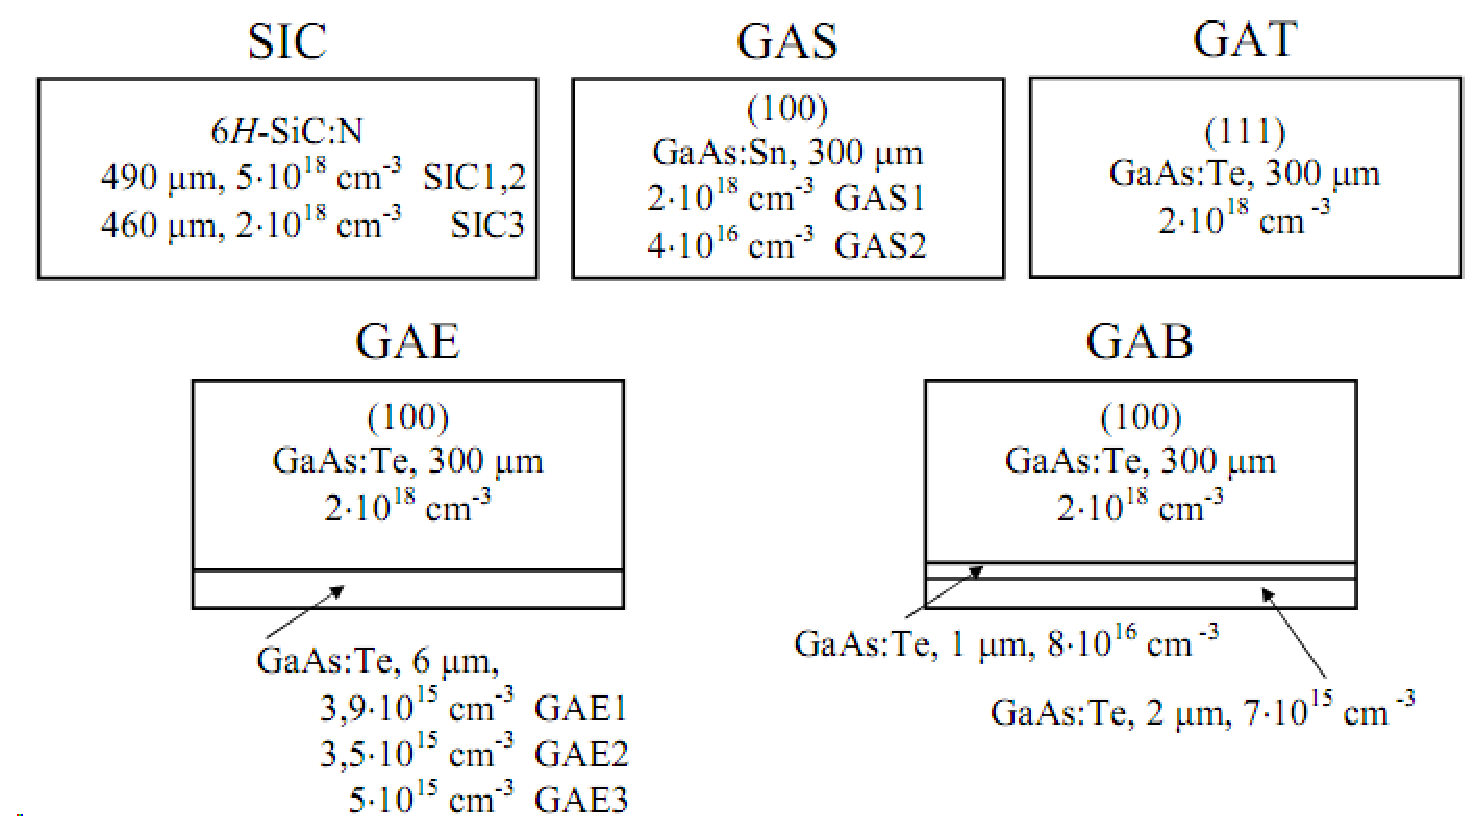
\includegraphics[width=0.5\textwidth]{Fig1}
\caption{\label{figSamp_TAV}
\hl{Schematic structure of the samples} for deep level investigations
}%
\end{figure}

The MWTs of the samples were performed in free space at room temperature in a magnetron at a frequency of  $\nu=2.45$~GHz
and specific power of $1.5$~W/cm$^{2}$.
The epitaxial structures were irradiated onto the side of the epitaxial layer.
The total exposure time $t_\mathtt{MWT}$ varied in the range of $20-80$~s for the different samples.
To avoid essential heating, the maximum single irradiation exposure time was no more than  five seconds.

The parameters of defects, such as the capture cross section of electron $\sigma_n$
and the energy level with respect to the conductivity band bottom $(E_c-E_t)$ were determined both before and after MWT.
%The parameters of deep centers, such as the efficient cross section of electron capture $\sigma_n$
%and location of the center energy level with respect to the conductivity band bottom $(E_c-E_t)$ were determined before and after MWT.
For this purpose, we used acoustoelectric transient spectroscopy \cite{OstrovPAN,OlikhSSC,PANnewEn,OstrovskiiSST}.
A schematic representation of this method is shown in \fref{figTAV}.
The samples were placed on a LiNbO$_3$ piezoelectric plate in which acoustic waves were excited as impulses.
After ultrasound impulse termination, relaxation of the transverse  acoustoelectric voltage (TAV) occurs according to
\begin{equation}\label{eqVtav}
  V_\mathtt{TAV}(t)=V_{\mathtt{TAV},0}\exp(-t/\tau).
\end{equation}

\begin{figure}
\includegraphics[width=0.5\textwidth]{fig2}
\caption{\label{figTAV}
Scheme of TAV signal  measurements.
Time dependence of radio impulse $V_\mathtt{RF}$ of ultrasound excitation in piezoelectric plate and the resulting TAV signal $V_\mathtt{TAV}$ are shown schematically
}%
\end{figure}

A simple exponential dependence according to equation~\eref{eqVtav} is observed in cases where only one type of trap is effective in acoustoelectric interactions.
For $n$-type semiconductors, the characteristic relaxation time is described by the equation \cite{OstrovPAN,OstrovskiiSST}
\begin{equation}\label{eqPANtau}
  \tau=\frac{1}{\sigma_n\,\upsilon_{\mathrm{th},n}\,N_c}\exp\left(\frac{E_c-E_t}{kT}\right),
\end{equation}
where
$\upsilon_{\mathrm{th},n}$ is the electron thermal velocity and
$N_c$ is the density of states in the conduction band.



The experimental measurements of the TAV relaxation at different temperatures and further approximation according
to equation~\eref{eqVtav}
allowed us to obtain the $\tau(T)$ dependence.
$(E_c-E_t)$ was determined from the slope of $\tau$ dependence on $(kT)^{-1}$ in semi-logarithmic scale
and then, using equation~\eref{eqPANtau}, $\sigma_n$ was calculated.
The measurements were performed in the temperature range $(290-350)$~K except for the GAB samples,
the TAV for which was high enough to be measured only after heating to above 310~K.

For single--crystal samples  before and after MWT, we also determined the curvature radius $R_\mathrm{cur}$
and deformation $\xi_\mathrm{cur}$ of the near-surface crystallographic planes.
The value of  $\xi_\mathrm{cur}$ was estimated by the X-ray method from the change in the angle of the diffraction
maximum location  during sample translation \cite{Godwod},
and the curvature was measured using a profilometer DekTak 3030 Veeco Instruments.
$R_\mathrm{cur}$ and $\xi_\mathrm{cur}$ were measured with a relative error no more than 2~\%.
For GaAs single crystals, we also analyzed the distribution of structural defects
over the area by using the Borman X-ray projection topography method,
and estimated the distribution of dislocation  densities and microstresses from the
analysis of the intensities of the Friedel reflection pairs $hkl$ and $hk$\emph{\={l}}.

\section{Results and discussion}\label{sec:Rez}

%\Fref{figTauTAV} presents the typical temperature dependencies of $\tau$ for the samples before and after the MWT.
%The above data show the change not only in the curve slopes (which is related to the level location in the gap),
%but also in the absolute value of the characteristic time of the relaxation TAV after MWT.
%The character of the MWT impact (the decrease or increase in relaxation time) depends not only on the exposure time and degree of doping but also on the internal structure of the samples under study.
%The results are presented in \tref{tabMW}.
%In the silicon carbide samples, there are two deep levels, labeled ESC1 and ESC2, while in gallium arsenide, there are six (EGA1–EGA6).

\Fref{figTauTAV} presents the typical temperature dependencies of $\tau$ for the samples before and after the MWT.
The above data show the MWT-induced change not only in the curve slopes (which is related to the level location in the gap),
but also in the absolute value of the characteristic time of the TAV relaxation.
The MWT impact depends not only on the exposure time and doping level but also on the internal structure of the samples under study.
\hl{The summary of the trap parameters detected in the samples} is presented in \tref{tabMW}.
In the silicon carbide samples, there are two deep levels, labeled ESC1 and ESC2, while in gallium arsenide, there are six (EGA1–EGA6).

\begin{figure*}
\center
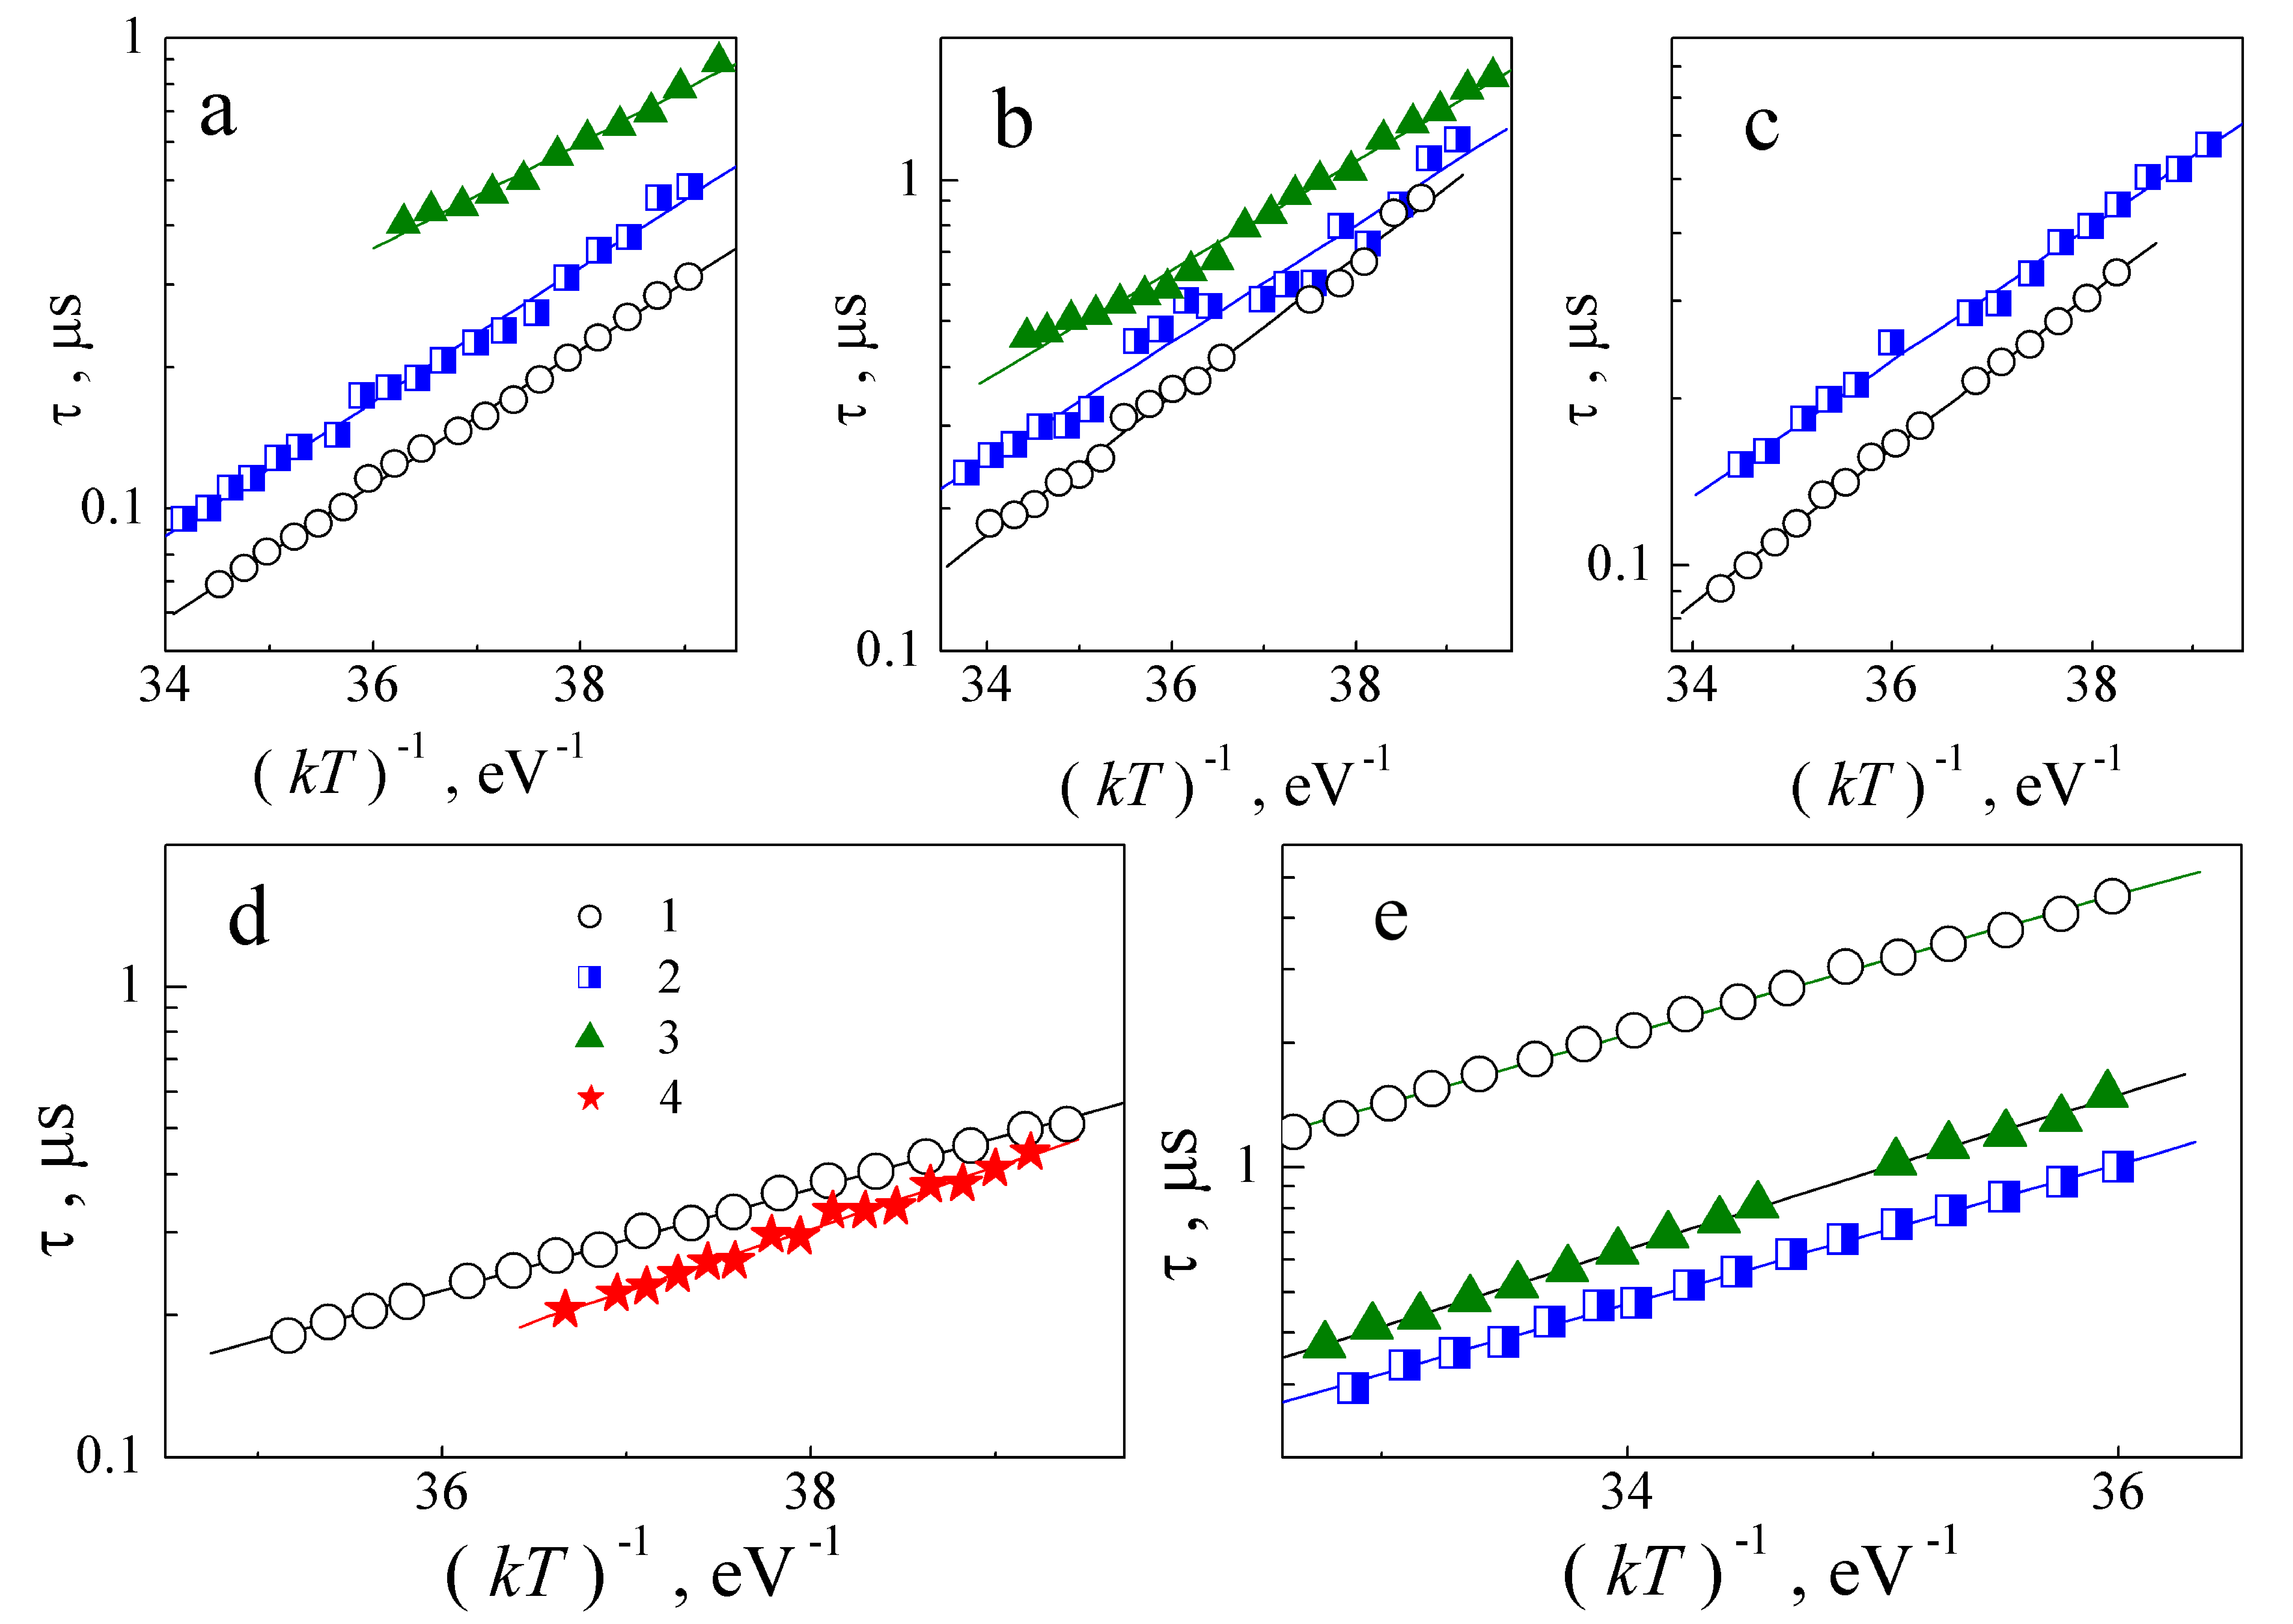
\includegraphics[width=0.7\textwidth]{Fig3}
\caption{\label{figTauTAV}
Dependencies of TAV relaxation time on inverse temperature for samples SIC2 (a), SIC3 (b), GAS2 (c), GAE2 (d) and GAB1 (e) before and after MWT.
$t_\mathtt{MWT}$, s: 0 (curves 1), 20 (2), 40 (3), 60 (4)
}%
\end{figure*}



\begin{table*}
\caption{\label{tabMW}
The determined defect parameters in samples $n$--GaAs and $n$--6$H$--SiC
}
\begin{indented}
\item[]\begin{tabular*}{\textwidth}{@{}*{7}{@{\extracolsep{0pt plus12pt}}c}}
\br
Sample& $t_{\rm MWT}$, s &Level &$(E_c-E_t)$, eV &$\sigma_n$, cm$^2$ $^{\rm a}$&$R_\mathrm{cur}$, m&$\xi_\mathrm{cur}$\\
\mr
SIC1& 0 &ESC1& $0.33\pm0.01$ &$(7\pm4)\times10^{-18}$&$\infty$&0\\ %\cline{2-7}
& 20 &ESC1& $0.33\pm0.01$ &$(5\pm3)\times10^{-19}$&170.2&$8.7\times10^{-7}$\\ %\cline{2-7}
& 40 &ESC2& $0.26\pm0.01$ &$(2\pm1)\times10^{-19}$&\multicolumn{2}{c}{\multirow{2}{*}{-}}\\ %\cline{2-5}
& 80 & \multicolumn{3}{c}{weak signal}&\multicolumn{2}{c}{}\\ %\hline
SIC2& 0 &ESC1& $0.33\pm0.01$ &$(7\pm4)\times10^{-18}$&$>2000$&$<1.2\times10^{-7}$\\ %\cline{2-7}
& 20 &ESC1& $0.33\pm0.01$ &$(5\pm3)\times10^{-19}$&171.9&$1.4\times10^{-6}$\\ %\hline
SIC3& 0 &ESC1& $0.34\pm0.02$ &$(3\pm2)\times10^{-18}$&3.8&$6.1\times10^{-5}$\\ %\cline{2-7}
& 20 &ESC2&$0.29\pm0.01$ &$(5\pm3)\times10^{-19}$&5.5&$4.2\times10^{-5}$\\ %\cline{2-7}
& 40 &ESC2& $0.26\pm0.01$ &$(10\pm7)\times10^{-20}$&\multicolumn{2}{c}{\multirow{2}{*}{-}}\\ %\cline{2-5}
& 80 &ESC2& $0.23\pm0.01$ &$(6\pm4)\times10^{-20}$&\multicolumn{2}{c}{}\\ %\hline
GAS1& 0 &EGA1& $0.32\pm0.02$ &$(3\pm2)\times10^{-17}$&-53.8&$-2.8\times10^{-6}$\\ %\cline{2-7}
& 20 &EGA1& $0.31\pm0.01$ &$(2\pm1)\times10^{-17}$&22.9&$6.5\times10^{-6}$\\ %\cline{2-7}
& 40 & \multicolumn{3}{c}{weak signal}&\multicolumn{2}{c}{-}\\ %\hline
GAS2& 0 &EGA1& $0.32\pm0.01$ &$(4\pm2)\times10^{-17}$&17.2&$8.7\times10^{-6}$\\ %\cline{2-7}
& 20 &EGA2& $0.28\pm0.01$ &$(5\pm2)\times10^{-18}$&14.7&$1.0\times10^{-5}$\\ %\cline{2-7}
& 40 & \multicolumn{3}{c}{weak signal}&\multicolumn{2}{c}{}\\ %\cline{1-5}
GAT& 0 &EGA3& $0.49\pm0.02$ &$(5\pm3)\times10^{-14}$&\multicolumn{2}{c}{}\\ %\cline{2-5}
& 20 &EGA4& $0.40\pm0.02$ &$(2\pm1)\times10^{-15}$&\multicolumn{2}{c}{}\\ %\cline{1-5}
GAE1& 0 &EGA5& $0.24\pm0.01$ &$(2\pm1)\times10^{-18}$&\multicolumn{2}{c}{}\\ %\cline{2-5}
& 60 &EGA2& $0.29\pm0.01$ &$(10\pm6)\times10^{-18}$&\multicolumn{2}{c}{}\\ %\cline{1-5}
GAE2& 0 &EGA5& $0.25\pm0.01$ &$(2\pm1)\times10^{-18}$&\multicolumn{2}{c}{}\\ %\cline{2-5}
& 60 &EGA2& $0.30\pm0.01$ &$(2\pm1)\times10^{-17}$&\multicolumn{2}{c}{}\\ %\cline{1-5}
GAE3& 0 &EGA6& $0.43\pm0.01$ &$(8\pm5)\times10^{-17}$&\multicolumn{2}{c}{-}\\ %\cline{2-5}
& 60 &EGA6& $0.46\pm0.02$ &$(7\pm4)\times10^{-16}$&\multicolumn{2}{c}{}\\ %\cline{1-5}
GAB1& 0 &EGA4& $0.39\pm0.01$ &$(10\pm7)\times10^{-18}$&\multicolumn{2}{c}{}\\ %\cline{2-5}
& 20 &EGA4& $0.39\pm0.01$ &$(4\pm2)\times10^{-17}$&\multicolumn{2}{c}{}\\ %\cline{2-5}
& 40 &EGA6& $0.43\pm0.02$ &$(10\pm6)\times10^{-17}$&\multicolumn{2}{c}{}\\ %\cline{1-5}
GAB2& 0 &EGA4& $0.40\pm0.01$ &$(10\pm6)\times10^{-17}$&\multicolumn{2}{c}{}\\ %\cline{2-5}
& 20 &EGA4& $0.41\pm0.01$ &$(10\pm6)\times10^{-17}$&\multicolumn{2}{c}{}\\ %\cline{2-5}
& 40 &EGA6& $0.45\pm0.02$ &$(4\pm2)\times10^{-16}$&\multicolumn{2}{c}{}\\  %\hline
\br
\end{tabular*}
\item[] $^{\rm a}$ at $T=300$~K for SIC, GA, GAE and at $T=340$~K for GAB
\end{indented}
\end{table*}

%The presented data show a number of characteristic features:
The presented results have several features:

\noindent
%i)~The value of the carrier capture cross section is much more sensitive to the MWT than the energy location of the levels.
%For example, $\sigma_n$ was found to change by an order of magnitude when the level location displacement was no more than 20\%, and
%the capture cross section was modified at lower exposition times.
%For instance, the value of $(E_c-E_t)$ for GAB1 practically did not change after 20~s of MW exposure, whereas $\sigma_n$ grew approximately four times.
i)~The capture cross section is much more sensitive to the MWT influence than the level energy.
For example, $\sigma_n$ was found to change by an order of magnitude when the level shift was no more than 20\%; besides, the lower exposition time was needed to change the capture cross-section.
For instance, the $(E_c-E_t)$ in GAB1 practically did not change after 20~s of MW exposure, whereas $\sigma_n$ grew approximately four times.

\noindent
%ii)~In single crystals, the  MWT-induced changes become stronger as the free charge carrier concentration decreases
%(see data on samples GAS1 and GAS2) and the relative deformation increases (the increase in surface curvature).
ii)~In single crystals, the  MW-induced changes become stronger
with a decrease in free charge carrier concentration
(see  GAS1 and GAS2 data)
and an increase in the relative deformation (the surface curvature).

\noindent
%iii)~After durable MWT of single-crystal samples ($t_{\rm MWT}>40$~s for GaAs,  $t_{\rm MWT}>80$~s for SiC),
%the TAV signal essentially decreased.
%This fact correlates with the data  from \cite{Belyaev1998JTFEn},
%who reported a decrease in the concentration of centers with levels in the upper half of the band gap as a result of MW annealing.
iii)~The durable MWT of single-crystal samples ($t_{\rm MWT}>40$~s for GaAs,  $t_{\rm MWT}>80$~s for SiC)
leads to an essential decrease in TAV signal magnitude.
This fact correlates with the data  from \cite{Belyaev1998JTFEn},
who reported a decrease in the concentration of centers with levels in the upper half of the band gap as a result of MW annealing.

\noindent
iv)~The irradiation dose required to essentially change the parameters of the trap
in the epitaxial structures was higher than one in single-crystal samples.
%The irradiation dose required to essentially change the parameters of the centers in the epitaxial structures was higher than that required for single-crystal samples.
In particular, \tref{tabMW} provides  data for the GA and GAB series samples after 20~s of MWT
which supports this fact.
Notably, the doping levels of  the GAB and GAE substrates were the same as those of samples GAS1 and GAT,
and the doping level of the GAB epitaxial layer was similar to that of GAS2.
In addition, GAB, GAE, and GAT contain the same doping impurities.
%Thus, the observed differences were determined by the structure of the samples but not by the difference in their conductivities.
Thus, the observed differences were determined by the sample's structures
but not by the difference in their conductivities.

\noindent
%v)~The characteristics of changes in single-crystal wafers and epitaxial structures are opposite:
%for SIC, GAS, GAT, $\sigma_n$ and $(E_c-E_t)$ were found to decrease after MWT,
%while for GAE and GAB, both parameters increased.
v)~If $t_{\rm MWT}$ is not enough to change the level location,
the MW-induced changes in the capture cross section are opposite
for SiC single-crystal and GaAs epi-structures.
In fact,  $\sigma_n$ were found to decrease in SIC1 and SIC2,
while for GAE and GAB, the capture cross section increased.


We now consider the possible configurations of the defects detected in the structures under study.
For this purpose, we should take into account that the reported data for the main trap parameters vary over a wide range;
in particular, the difference between the values of capture cross sections can be as large as four orders of magnitude \cite{Pavlovic2000}.
One of the possible reasons for such a large spread of parameters is the strong
dependence of the charge thermal emission on the electric field strength \cite{Bulyarskii2000,Makram} caused by
a)~decrease in ionization energy due to the Pool--Frenkel effect or, for example, Coulombic interactions of defect \cite{Stellmacher} and
b)~change in the $\sigma_n$  magnitude \cite{Bourgoin2001}.
As a rule, the change in $(E_c-E_t)$ comprises several tens of meV, and
the change in the capture cross-section reaches several orders of magnitude.
For instance, according to Bourgoin and Angelis \cite{Bourgoin2001}, at room temperature,
$\sigma_n$  for the $EL2$ center in GaAs decreases 200 times
at an intensity of $10^5$~V/cm.
Consequently, the different methods used to investigate defects yield  different parameters for the same centers.
For example, from reviews on various traps in gallium arsenide,  we can compare the data  obtained by deep-level transient spectroscopy \cite{Bourgoin:GaAs}
and thermally stimulated currents \cite{Pavlovic2000}.
Data were obtained for defects with closely located levels and very different capture cross section values.
%Generalizing the above-mentioned, we should note that it is the energy location of traps that we shall be oriented towards in our research.
Generalizing the above-mentioned, we should note that it is the energy \hl{level that
we shall be oriented towards in defect configuration determination.
If the change in $(E_c-E_t)$ after MWT has exceeded the experimental errors limit (about 20~meV),
we supposed the microwave-induced configuration change.}

The position of the ESC1 level ($E_c-(0.33-0.34)$~eV) observed in the initial SiC crystals can be compared
with the position of the $S$--center ($E_c-0.35$~eV) \cite{Lebed1999En,Anikin1991:2En,Anikin1991:3En},
EK–center ($E_c-0.34$~eV) \cite{Kuznets1997En},
or $(-/+)$ level $E1$ ($E_c-0.34$~eV) \cite{Lebed1999En}.
$S$--center is responsible for non-radiative recombination, and
in 6$H$–SiC it is a self-interstitial defect \cite{Lebed1999En}.
According to the \cite{Anikin1991:2En,Anikin1991:3En},
the $S$--center and $R$--center ($E_c-1.27$~eV) are associated with two different charge states
of the same defect,
whereas according to Lebedev~\etal. \cite{Lebedev2000En},
the $R$--center is a divacancy $\mathrm{V}_\mathrm{Si}\mathrm{V}_\mathrm{C}$.
It should be noted that  a divacancy is a typical defect in 6$H$--SiC \cite{SiCBaran,SiCDavid}.
On the other hand, the level $E_c-0.39$~eV is more often associated with center $E1$ \cite{SiCWei,SiCKoizumi}.
Thus, in our opinion, ESC1 level is related to complex $\mathrm{V}_\mathrm{Si}\mathrm{V}_\mathrm{C}$.

%After the MWT, the position of the level responsible for TAV generation in SiC shifted to $E_c-(0.26-0.29)$~eV (level ESC2).
After the MWT, the level of the trap,
which is responsible for TAV arising in SiC,
shifted to $E_c-(0.26-0.29)$~eV (level ESC2).
This situation is also ambiguous: closely located are donor level $(0/+)$ of
center $E1$ ($E_c-(0.27-0.28)$~eV \cite{Hemmingsson},
$E_c-0.26$~eV \cite{SiCWei,SiCKoizumi}
and center $X1$ ($E_c-0.3$~eV) \cite{Lebedev2001En}.
The authors of the latter publication reported the essential dependence of $X1$ concentration on crystal structural perfection.
They stressed that $X1$ was not identical to $E1$.
In turn, level $E1$ has been identified as the center of the negative
correlation energy \cite{Lebedev2001En,SiCWei}
and dominating intrinsic point defect in $n$--type 6$H$--SiC \cite{SiCSasaki}.
According to Refs.~\cite{SiCSasaki,SiCWei}, $E1$ is related to carbon vacancy.
Considering the difference between the $X1$ and ESC2 energy locations,
the configuration $\mathrm{V}_\mathrm{C}$ was associated with the ESC2 level.
\hl{In addition, the connection between the level $E_c-0.26$~eV and the carbon vacancy
is confirmed by Grossner}~\etal \cite{SiC:bookCh6}.

The data for levels revealed for gallium arsenide are listed in \tref{tabEGA1}.
The presented data show that the traps are associated with intrinsic vacancy-related defects:
\hl{EGA1 is V$_\mathrm{As}$,
EGA2 is V$_\mathrm{As}$As$_i$,
EGA3 is V$_\mathrm{As}$ or  V$_\mathrm{Ga}$Ga$_i$V$_{\rm As}$,
EGA4 is V$_\mathrm{Ga}$Ga$_\mathrm{As}$,
EGA5 is V$_\mathrm{Ga}$V$_\mathrm{As}$,
and EGA6 is V$_\mathrm{As}$As$_i$.}



\begin{table*}
\caption{\label{tabEGA1}
Data reported for the levels close to detected levels in GaAs samples
}
\begin{indented}
\item[]\begin{tabular*}{\textwidth}{@{}*{6}{@{\extracolsep{0pt plus12pt}}c}}
\br
$(E_c-E_t)$, eV &$\sigma_n$, cm$^2$&configuration&method$^{\rm a}$&epi--structure&Reference\\
\mr
\multicolumn{6}{c}{EGA1, ($E_c-E_t)=(0.31-0.32)$~eV}\\
0.33&-&complex with V$_\mathrm{As}$&DLTS&no&\cite{EL6:Richter}\\% \hline
0.33&-&-&DLTS&no&\cite{Neild1991}\\ %\hline
$0.31-0.33$&-&V$_\mathrm{As}$&LDA&no&\cite{EL6:Schultz}\\ %\hline
0.33&$1\times10^{-17}$&-&TSC&no&\cite{Pavlovic2000}\\ %\hline
0.323&$1\times10^{-14}$&-&DLTS&yes&\cite{Yousefi1995}\\ %\hline
0.334&$2\times10^{-15}$&&DLTS&yes&\cite{Yousefi1995}\\ %\hline
0.35&-&complex with V$_\mathrm{As}$&PA&no&\cite{EL6:Kuisma}\\ %\hline
$0.315-0.325$&$3\times10^{-17}$&-&TSC&no&\cite{Pavlovic:GaAs}\\ %\hline
0.33&-&-&TSC&no&\cite{Tomozane:GaAs}\\ %\hline
$0.30-0.33$&-&-&DLTS&no&\cite{Lang:GaAs}\\ %\hline
\multicolumn{6}{c}{EGA2, ($E_c-E_t)=(0.28-0.30)$~eV}\\
0.28&$5\times10^{-18}$&V$_\mathrm{As}$As$_i$&TSC&no&\cite{Pavlovic2000}\\ %\hline
0.26&$3.5\times10^{-15}$&-&DLTS&yes&\cite{Yousefi1995}\\ %\hline
%0.277&$5\times10^{-17}$&-&TSC&no&\onlinecite{Pavlovic:GaAs}\\ %\hline
0.30&-&intrinsic&DLTS&no&\cite{PhysRevB1986}\\ %\hline
0.284&$1\times10^{-17}$&-&TSC&no&\cite{Pavlovic:GaAs}\\ %\hline
0.28&-&intrinsic&TP&no&\cite{Abele:GaAs}\\ %\hline
0.28&$8\times10^{-15}$&-&DLTS&yes&\cite{Mircea1975}\\ %\hline
0.30&-&complex with Te&DLTS&no&\cite{KolFTP1994En}\\ %\hline
0.30&$6\times10^{-15}$&V$_\mathrm{As}$As$_i$&DLTS&no&\cite{Pons}\\ %\hline
\multicolumn{6}{c}{EGA3, ($E_c-E_t)=0.49$~eV}\\
0.50&-&Sb$_\mathrm{Ga}$&DLTS&no&\cite{Samoilov1994En}\\ %\hline
0.48&$4\times10^{-16}$&As$_\mathrm{Ga}^{++}$&TSC&no&\cite{Pavlovic2000}\\ %\hline
0.485&$2\times10^{-16}$&-&TSC&no&\cite{Pavlovic:GaAs}\\ %\hline
0.48&-&impurity&TP&no&\cite{Abele:GaAs}\\ %\hline
%0.51&$1\times10^{-12}$&-&DLTS&no&\onlinecite{Martin1977}\\ %\hline
0.49&$2\times10^{-13}$&impurity+V$_\mathrm{As}$&DLTS&yes&\cite{GaAsBlood}\\ %\hline
0.48&$3\times10^{-13}$&-&DLTS&no&\cite{Lang:GaAs}\\ %\hline
0.50&$1\times10^{-15}$&V$_\mathrm{As}$, V$_\mathrm{Ga}$Ga$_i$V$_\mathrm{As}$ &DLTS&no&\cite{Pons}\\
\multicolumn{6}{c}{EGA4, ($E_c-E_t)=(0.39-0.41)$~eV}\\
0.42&-&-&DLTS&no&\cite{Neild1991}\\ %\hline
0.41&-&V$_\mathrm{Ga}$V$_\mathrm{As}$&DLTS&no&\cite{Samoilov1994En}\\ %\hline
$0.39$&-&V$_\mathrm{Ga}$Ga$_\mathrm{As}$&TSC&no&\cite{FANG1990}\\ %\hline
$0.41$&$2\times10^{-13}$&-&DLTS&yes&\cite{Bourgoin:GaAs}\\ %\hline
0.40&-&-&SCRC&yes&\cite{ASHBY:GaAs}\\ %\hline
0.37&$2\times10^{-14}$&-&DLTS&yes&\cite{Fang:EL6}\\ %\hline
0.40&-&V$_\mathrm{Ga}$Ga$_\mathrm{As}$&DLTS&no&\cite{VaitkusEn}\\ %\hline
0.387&$2\times10^{-14}$&-&DLTS&yes&\cite{Yousefi1995}\\ %\hline
\multicolumn{6}{c}{EGA5, ($E_c-E_t)=(0.24-0.25)$~eV}\\
0.23&-&-&DLTS&no&\cite{Neild1991}\\ %\hline
0.23&$2\times10^{-17}$&-&TSC&no&\cite{Pavlovic2000}\\ %\hline
$0.22-0.25$&$8\times10^{-19}$&-&TSC&no&\cite{Lin:GaAs}\\ %\hline
$0.26$&-&complex with V$_\mathrm{Ga}$&TSC&no&\cite{FANG1990}\\ %\hline
0.24&-&-&TSC&no&\cite{Tomozane:GaAs}\\ %\hline
0.23&-&intrinsic&TP&no&\cite{Abele:GaAs}\\ %\hline
0.23&-&V$_\mathrm{Ga}$V$_\mathrm{As}$&DLTS&no&\cite{Morrow:EL17}\\ %\hline
0.23&$1\times10^{-14}$&V$_\mathrm{Ga}$V$_\mathrm{As}$&DLTS&no&\cite{Bourgoin:GaAs}\\ %\hline
0.23&$7\times10^{-15}$&-&DLTS&yes&\cite{Mircea1975}\\ %\hline
%0.22&$2\times10^{-15}$&-&DLTS&no&\onlinecite{Fang:EL6}\\ %\hline
0.236&$1\times10^{-16}$&complex with V$_\mathrm{As}$&DLTS&yes&\cite{GaAsBlood}\\ %\hline
0.258&$4\times10^{-16}$&-&DLTS&yes&\cite{Yousefi1995}\\ %\hline
\multicolumn{6}{c}{EGA6, ($E_c-E_t)=(0.43-0.46)$~eV}\\
0.44&$1\times10^{-14}$&V$_\mathrm{As}$As$_i$, V$_\mathrm{As}$&TSC&no&\cite{Pavlovic2000}\\ %\hline
0.44&$9\times10^{-15}$&-&TSC&no&\cite{Pavlovic:GaAs}\\ %\hline
\multirow{2}{*}{0.43}&\multirow{2}{*}{$7\times10^{-16}$}&\multirow{2}{*}{intrinsic}&\multirow{2}{*}{DLTS}&\multirow{2}{*}{yes}&\cite{Lefevre1977}\\
&&&&&\cite{Bourgoin:GaAs}\\
%0.43&$7\times10^{-16}$&intrinsic&DLTS&yes&\onlinecite{Lefevre1977} \onlinecite{Bourgoin:GaAs}\\ %\hline
0.44&$2\times10^{-15}$&complex with V$_\mathrm{As}$&DLTS&yes&\cite{KolFTP1989En}\\ %\hline
\br
\end{tabular*}
\item[] $^{\rm a}$ DLTS --- deep level transient spectroscopy;
TSC --- thermally stimulated current; LDA --- local density approximation;
PA --- positron annihilation techniques;
TP --- photoinduced transient spectroscopy;
SCLC --- space charge limited current
\end{indented}
\end{table*}

Several factors caused the trap parameters to change.
They are as follows.

\noindent
i)~Transformation of the defect complex due to decay, involvement of additional components, change in the distance between defect components, etc.

\noindent
ii)~Defect recharging.

\noindent
iii)~Changes in the trap environment, which can result, for instance, in the modified strength of the electric field around the defect.

\noindent
iv)~An increase in the concentration of a given type of defect;
for instance, the change in ionization energy was reported \cite{Stellmacher} to be proportional to the cubic root of the defect concentration.

Analysis of the observed phenomena should consider
the probable mechanisms of the impact of microwave radiation on the crystals.
First, the effect of the temperature increase should be analyzed.
It is believed that the structural modification in the MWT result  is mostly caused by the change
in the defect charge state and elastic stress fields arising in instantly heated defect regions.
However, these processes are known to intensify with increasing free charge carrier concentrations \cite{MW:Rev},
whereas in our case, the effects weaken with the concentration increase (samples GAS1 and GAS2).
Moreover, the applied irradiation mode did not imply long-term continuous exposure to MW oscillations,
which reduced the overall heating of the structure.
However, numerous studies have shown that the observed effects of MWT cannot be explained only by the mechanisms of fast  annealing;
therefore, non-thermal factors should also be considered.
In recent research, more attention has been paid to the non-thermal mechanisms of MWT action
(see, for example, \cite{MW:Si2018} and the references it contains),
which cause dislocation generation and result in smaller  clusters of point defects in semiconductor wafers \cite{Konakova2007JTFEn}
or even trigger recrystallization processes \cite{MW:Si2018}.
Possible non-thermal processes causing changes in the structural characteristics of binary semiconductors have been reported in \cite{Konakova2007JTFEn}.
In particular, the processes of dislocation oscillations under the action of an electric field were analyzed,
and the decorating impurities were found to influence the behavior of the dislocation segments.
On the one hand, the available impurities decrease the resonance frequency of oscillations
and provide the presence of electric charge,
on the other hand, at high oscillation amplitudes they can escape the dislocation,
which causes new chemical defects to arise.
In turn, the point defects can perform superhigh-frequency oscillations and diffuse as a result of the MWT.

The observed modifications of deep-level parameters are the result of the above-mentioned
structural reconstruction in semiconductor near-surface regions  owing to the MWT.
The results of X--ray investigations show that MWT increases the convexity of single-crystal samples,
which indicates the aggregation of interstitial defects in the near-surface layer,
particularly because of the generation of separate dislocations \cite{BoltovetsEn,Konakova2012FTPEn}.
The defect accumulation effect caused by the MWT in the near-surface region  was reported in \cite{BoltovetsEn,Konakova2015En}.
To a certain extent, only the SIC3 sample was excluded;
however in this case, a rather strong deformation of the near-surface region was also observed prior to irradiation.
Researchers have reported \cite{Bacherikov2003En,Pashkov1994En,BoltovetsEn,Milenin1994En,BelyaevIntac} that in this stressed state,
MWT causes redistribution as well as certain weakening of elastic deformations, which is what occurs in SIC3.
The profilometry data correlated with X--ray measurements.
Structural investigations show that
in the initial GaAs samples, the density of dislocations has a W-like distribution over the plate area; the dislocation density over the plate diameter varied from $2\cdot10^{4}$~cm$^{-2}$ to $2\cdot10^{5}$~cm$^{-2}$.
This inhomogeneity in the dislocation density distribution is evidence of  considerably strong elastic deformation in the sample.

The analysis showed that the ESC1 and ESC2 centers are complexes of carbon vacancies,
EGA1 is associated with V$_\mathrm{As}$,
and EGA3 — with V$_\mathrm{As}$ or  V$_\mathrm{Ga}$Ga$_i$V$_{\rm As}$ complexes.
The MWT stimulates the diffusion of point defects, which are mostly intrinsic interstitial atoms, resulting in trap modifications.
The ESC1 center in silicon carbide transforms into ESC2 under the influence of closely located interstitial silicon:

\begin{equation*}
\mathrm{V}_\mathrm{Si}\;\mathrm{V}_\mathrm{C}+\mathrm{Si}_{\,i} \rightarrow
   \mathrm{V}_\mathrm{C}\,.
\end{equation*}

Further modification of the ESC2 parameters in SIC3 is caused by the enhanced electric field of the dislocation.
In the GAS2 samples at $t_\mathrm{MWT}=20$~s,
the V$_\mathrm{As}$ transformed into complex V$_\mathrm{As}$As$_i$
(EGA2 center)
because of the increased number of interstitial atoms in the near-surface layer:
\begin{equation*}
\mathrm{V}_\mathrm{As}+ \mathrm{As}_{\,i} \rightarrow \mathrm{V}_\mathrm{As}\;\mathrm{As}_{\,i}\,.
\end{equation*}

A similar process in GAS1 is more complicated because of its higher charge carrier concentration.
It has been reported \cite{ZOHM2000} that with a growth in resistance, the depth of microwave penetration increases,
and thus, the volume from which defect gettering begins in the near-surface layer grows as well.
In addition, the cause of the weak (in comparison with GAS2) influence of MWT on trap parameters in GAS1 is the absence of pressure stresses,
which intensifies the MWT-simulated complex formation process in the system’s intrinsic defects.
This is supported by data for silicon carbide single crystals.
In the GAT sample, which is also characterized by a high concentration of free electrons,
the transformation of EGA3 to EGA4 (V$_\mathrm{Ga}$Ga$_\mathrm{As}$ complex) occurs in the reaction described in \cite{FANG1990}:
\begin{equation*}
  \mathrm{V}_\mathrm{Ga}\;\mathrm{Ga}_{\,i}\;\mathrm{V}_\mathrm{As}\rightarrow \mathrm{Ga}_\mathrm{Ga}\;\mathrm{V}_\mathrm{As}
  \rightarrow \mathrm{Ga}_\mathrm{As}\;\mathrm{V}_\mathrm{Ga}
\end{equation*}

Accumulation of a large number of interstitial atoms in the near-surface layer at high doses of radiation
($t_{\rm MWT}\approx40$~s for gallium arsenide and $t_\mathrm{MWT}>80$~s for silicon carbide)
causes complete annihilation of vacancies (or transformation into antisite defects, whose levels are filled in the crystals with electron conductivity);
 therefore, the TAV signal disappears (samples GAS1, GAS2, SIC1):
\begin{eqnarray}
  \nonumber
  \mathrm{SiC}&:&\mathrm{V}_\mathrm{Si}\;\mathrm{V}_\mathrm{Si}+\mathrm{Si}_{\,i}+ \mathrm{Si}_{\,i} \rightarrow 0\,;\\
  \nonumber
  \mathrm{GaAs}&:&\mathrm{V}_\mathrm{As}+\mathrm{As}_{\,i} \rightarrow 0\,;\quad
  \mathrm{V}_\mathrm{As}+\mathrm{Ga}_{\,i} \rightarrow \mathrm{Ga}_\mathrm{As}\,.
\end{eqnarray}

It is believed \cite{OstrovskiiSST,OlikhSSC,OstrovPAN} that the TAV
that arises in epitaxial structures
is mostly caused by defects located at the epi--layer and substrate interface.
This difference in the deep-level location
is the cause of the difference between the dose-dependent modification of the defect parameters in the epitaxial and single-crystal samples.

In epitaxial structures $n$--$n^+$--GaAs and $n$--$n^+$--$n^{++}$--GaAs,
MWT induced increase of curvature radius reported in \cite{BoltovetsEn,Konakova2012FTPEn}
is the result of forming single dislocations and their further propagation deep into the structure along the glide planes.
As a result, the strength of both the electric and stress fields changes,
which causes defect transformation and, thus, the shift of the respective deep levels.
As shown in \tref{tabEGA1}, EGA5 and EGA6 levels were associated with the complexes   V$_\mathrm{Ga}$V$_\mathrm{As}$  and V$_\mathrm{As}$As$_i$, respectively.
Traps such as EGA2 and EGA4 have also been previously found in epi-structures \cite{Yousefi1995,Mircea1975,Bourgoin:GaAs,ASHBY:GaAs,Fang:EL6,Lefevre1977,KolFTP1989En}.
The observed MWT-stimulated transformations are caused by an increasing number of interstitial atoms, which are described by the following reactions: \begin{equation*}
  \mathrm{V}_\mathrm{Ga}\;\mathrm{V}_\mathrm{As}+\mathrm{Ga}_{\,i}+\mathrm{As}_{\,i} \rightarrow \mathrm{V}_\mathrm{As}\;\mathrm{As}_{\,i}
\end{equation*}
for GAE1 and GAE2 and
\begin{equation*}
  \mathrm{V}_\mathrm{Ga}\;\mathrm{Ga}_\mathrm{As}+\mathrm{As}_{\,i} \rightarrow
  \mathrm{Ga}_\mathrm{Ga}\;\mathrm{V}_\mathrm{As}+\mathrm{As}_{\,i} \rightarrow
  \mathrm{V}_\mathrm{As}\;\mathrm{As}_{\,i}
\end{equation*}
for GAB1 and GAB2.
The increase in activation energy EGA6 in sample GAE3 is probably caused by the change in
Coulombic interaction of interstitial--vacancy complexes,
which is due to a decrease in their concentration,
while the growth of capture cross section EGA4 in GAB1 at $t_\mathrm{MWT}=20$~s
and EGA6 in GAE3 are associated with the growth of the electric field strength caused by charged dislocations.

\section{Conclusion}
The influence of microwave radiation on the parameters of point defects (cross section of electron capture and energy levels in the gap)
was studied experimentally  in single crystals of $n$–6$H$-SiC and  $n$–GaAs, as well as in gallium arsenide epitaxial structures.
The investigation showed that the traps available in the near-surface layer are associated with intrinsic
vacancy-related defects.
The microwave radiation-induced change in the trap energy level and capture cross section
was caused by the growing number of interstitial atoms in the near-surface layer.
The radiation-induced process involving the transformation of defect complexes intensifies under stress conditions.
Thus microwave processing can be an effective tool of defect engineering.

\section*{Data Availability Statement}

The data that support the findings of this study are available from the corresponding author upon reasonable request.

\section*{References}

\bibliographystyle{iopart-num}
\bibliography{olikh}

\end{document}

